
% This LaTeX was auto-generated from an M-file by MATLAB.
% To make changes, update the M-file and republish this document.

\documentclass{article}
\usepackage{graphicx}
\usepackage{color}

\sloppy
\definecolor{lightgray}{gray}{0.5}
\setlength{\parindent}{0pt}

\begin{document}

    
    \begin{verbatim}
%
% Autofocus
%

N = 1000;

% directory that contains the image sequence
img_dir = 'images';
% type of the image (e.g. jpg)
img_type = '.png';
img_names = dir([img_dir '/*' img_type]);
\end{verbatim}
\begin{par}
name of the first image
\end{par} \vspace{1em}
\begin{verbatim}
%img_name = img_names(1).name;

imshowD = @(img) imshow(im2uint8(img));
focVal = [];
focName = [];

for i = 1:length(img_names)
    img_name = img_names(i).name;
    img = imread([img_dir '/' img_name]);
    imgG = rgb2gray(img);
    imgG = im2double(imgG);

    %figure('name',img_name);
    %subplot(2,2,1);
    %imshowD(imgG)
    %subplot(2,2,2);
    [grd,~] = imgradient(imgG,'CentralDifference');
    %imshowD(grd / max(grd(1:end)));

    %subplot(2,2,3);
    %hist(grd(1:end),0:0.01:1);

    grdS = sort(grd,'descend');

    focusInd = sum(grdS(1:N)) / N;
    fprintf('%s - %d\n', img_name, focusInd);

    focVal = [focVal, focusInd];
end
\end{verbatim}

        \color{lightgray} \begin{verbatim}image_01.5.png - 5.770013e-03
image_01.75.png - 6.054750e-03
image_02.0.png - 6.610152e-03
image_02.5.png - 7.630068e-03
image_03.png - 8.679687e-03
image_04.png - 7.685592e-03
image_05.png - 7.312498e-03
image_07.5.png - 6.757971e-03
image_10.png - 6.505572e-03
image_inf.png - 5.801062e-03
\end{verbatim} \color{black}
    \begin{verbatim}
focNames = {};
for i = 1:length(img_names)
    n = img_names(i).name;
    focNames{i} = n(7:end-4);
end
\end{verbatim}
\begin{verbatim}
plot(focVal);
set(gca,'XLim',[1 length(focNames)],'XTick',1:length(focNames),'XTickLabel',focNames)
\end{verbatim}

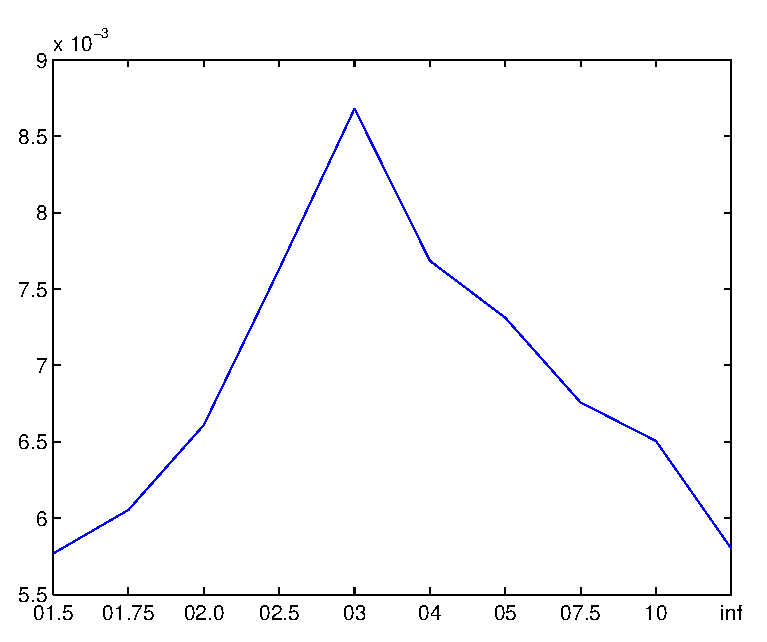
\includegraphics [width=4in]{main_01.eps}



\end{document}
    
